\chapter{Trading Strategies}
\label{sec:strats}
As previously mentioned, the strategies employed are variations of the mean reversion trading strategy. The basic concept of a mean reversion strategy identifies two closely related assets, typically referred to as a pair, and takes advantage of deviations from their historical price relationship. This works by initially identifying a pair of assets that have a historically stable relationship, as seen in Section \ref{sec:liquidity-pools}. Then as prices change, the spread between the prices is calculated, and if the spread has deviated from the historical mean spread, the strategy should buy the undervalued asset and sell the other. The positions are then closed once the spread reverts back to its historical mean.

\section{Abstract Strategy}
The implementation of the generalization of these strategies is intricate and designed to be scalable and highly customizable with various parameters. Additionally, since the trading strategies being investigated are based on mean reversion, an abstract strategy is created to allow for quick exploration and research into different approaches and the impact of hedge ratio calculations on returns. This abstract strategy encompasses the core logic of generating trading signals, determining optimal trade timing and volumes, and transmitting them to the live or backtesting system. The strategy-specific classes contain operations that calculate the hedge ratio and establish the thresholds that trigger the generation of trading signals. Below shows the functions that the abstract strategy possesses.
\begin{lstlisting}[language=Python]
class Abstract_Strategy():
    def __init__(self, number_of_sds_from_mean, window_size_in_seconds, percent_to_invest, strategy_name, gas_price_threshold, rebalance_threshold_as_percent_of_initial_investment):
        ...

    def initialise_historical_data(self, history_p1, history_p2):
        ...

    def recalculate_thresholds(self, has_trade=False):
        raise NotImplementedError("recalculate_thresholds not implemented")

    def new_tick(self, price_of_pair1, price_of_pair2, has_trade):
        ...

    def generate_signal(self, ctx, prices):
        ...

\end{lstlisting}

\noindent The functions \texttt{\_\_init\_\_,\ initialise\_historical\_data,\ new\_tick} and \texttt{generate\_signal} are all inheritted by each strategy and \texttt{recalculate\_thresholds} is implemented in each instance of the strategy. \texttt{\_\_init\_\_,\ initialise\_historical\_data} are self explanatory. \texttt{new\_tick} is called in \texttt{generate\_signal} to update the strategy's knowledge of historical prices; this function also triggers a call to \texttt{recalculate\_thresholds} which re-calculates the hedge ratio and determines the thresholds at which an arbitrage opportunity becomes apparent. \texttt{generate\_signal} is the function that is called by the trading system at each price update. It first invokes \texttt{new\_tick}, which in turn updates the thresholds; finally, the updated hedge ratio and thresholds are used in the process of generating a signal. The steps of \texttt{generate\_signal} are outlined below:
\begin{enumerate}
    \item The first step is to call \texttt{new\_tick} which updates the thresholds
    \item Second is to check whether a position is already held;
    \begin{enumerate}
        \item If a position IS held, the first is to check if the spread is between the thresholds, and if the gas price is below the specified limit, the positions are closed. However, before this, a precautionary check is made to ensure the balance of any token does not go below 0; if it does, a swap order is placed before the closing of the positions such that the balance of each token remains positive. Otherwise, the loan-to-value health factor is calculated; if it may cause liquidation, additional collateral is deposited in Aave.
        \item However, if a position is NOT held and the gas price is below the specified limit, there are 3 cases. \begin{enumerate}
            \item $spread > upper\_threshold$ - Buy pair 2 and sell pair 1
            \item $spread > lower\_threshold$ - Buy pair 1 and sell pair 2
            \item No trade
        \end{enumerate}
        Furthermore, if a trade is ordered, it is also checked; if the WETH balance falls below the rebalance threshold, the additional tokens are converted back to WETH.
    \end{enumerate}
    In addition, prior to opening or closing a position, a preliminary check is conducted to ensure that the ETH balance remains positive. If the anticipated balance after executing the orders indicates a potential shortfall, an order to \texttt{BUY\ ETH} is automatically initiated. This precautionary measure ensures that the strategy maintains a positive ETH balance and avoids entering into positions that could lead to negative balances.
\end{enumerate}
Refer to Appendix \ref{app:strats-hr-calcs} to see the implementations of calculating the hedge ratios of each strategy.

\subsection{Volume of Trades}
A major part of the strategy is at which volumes to trade; therefore, in order to be able to trade the maximum amount, a minimization problem must be solved. However, before delving into this problem, it is important to highlight the influence of the hedge ratio on the trading volumes. If the hedge ratio is positive, for every unit of pair0 traded, \texttt{hedge\_ratio} units of pair1 should be traded. However, the inverse is true if the hedge ratio is negative; for every \texttt{-hedge\_ratio} units of pair0 traded, 1 unit of pair1 should be traded.
\\[3mm]
Given that $Z$ is the amount of WETH in the account, $p_0, p_1$ are the prices of pairs 0 and 1 respectively, $LTV$ is the loan-to-value ratio and $x, y$ are the volumes to be traded on pair0 and pair1 respectively. Additionally, to generalize the problem for both positive and negative hedge ratios, let $n:k$ represent the ratio of volume traded for pair0:pair1. Assuming we are buying pair0 and selling pair1. The solution to the following minimization problem is used to find the maximum volumes that can be traded to leave the least amount of WETH remaining.
\begin{equation}
\begin{aligned}
\min_{x, y} \quad & Z - xp_0 - \frac{yp_1}{LTV}\\
\textrm{s.t.} \quad & x = \frac{k}{n}y\\
    &x, y \geq 0\\
    &p_0, p_1 \geq 0\\
    &Z \geq 0\\
    &0 \leq LTV \leq 1\\
\end{aligned}
\end{equation}
Therefore, as all terms in the objective function are positive, therefore, the minimal objective value, in theory, must be 0:
\begin{align*}
    Z - xp_0 - \frac{yp_1}{LTV} &= 0\\
    Z - \frac{k}{n}yp_0 - \frac{yp_1}{LTV} &= 0\\
    Z - (\frac{k}{n}p_0 + \frac{p_1}{LTV})y &= 0\\
    y &= \frac{Z}{\frac{k}{n}p_0 + \frac{p_1}{LTV}}\\
    x &= \frac{k}{n}\frac{Z}{\frac{k}{n}p_0 + \frac{p_1}{LTV}}
\end{align*}
\noindent Thus, the resulting values of $x$ and $y$ represent the solution that minimizes the problem while maximizing the tradable volume. The case above shows that $x$ units of pair0 can be bought, and thus $y$ units of pair1 must be sold. Similarly, if pair0 is sold and pair1 is bought, the maximum volumes are determined by $x = \frac{Z}{\frac{p_0}{LTV} + \frac{n}{k}p_1}$ and $y = \frac{n}{k} \frac{Z}{\frac{p_0}{LTV} + \frac{n}{k}p_1}$.

\section{Constant Hedge Ratio Strategy}
In the most simplistic mean reversion strategy, the approach relies on a given historical dataset, assuming that the hedge ratio between the paired assets remains consistent over the long term. To determine this hedge ratio, the Ordinary Least Squares (OLS) regression method is employed.
\\[3mm]
In Figure \ref{fig:f1}, the observed trend reveals that the gradient, representing the rate of change, exhibits proximity to the value of 1. This indicates a relatively balanced relationship between the prices of each pair. However, it is important to note that as time progresses, any fluctuations or deviations from the exact value of 1 are minimal and have a negligible impact on the overall trend. The stability of the gradient over time suggests a consistent and relatively stable relationship between the liquidity pools, reinforcing the notion that their interdependence remains relatively constant.
\begin{figure}[!htb]
    \centering
    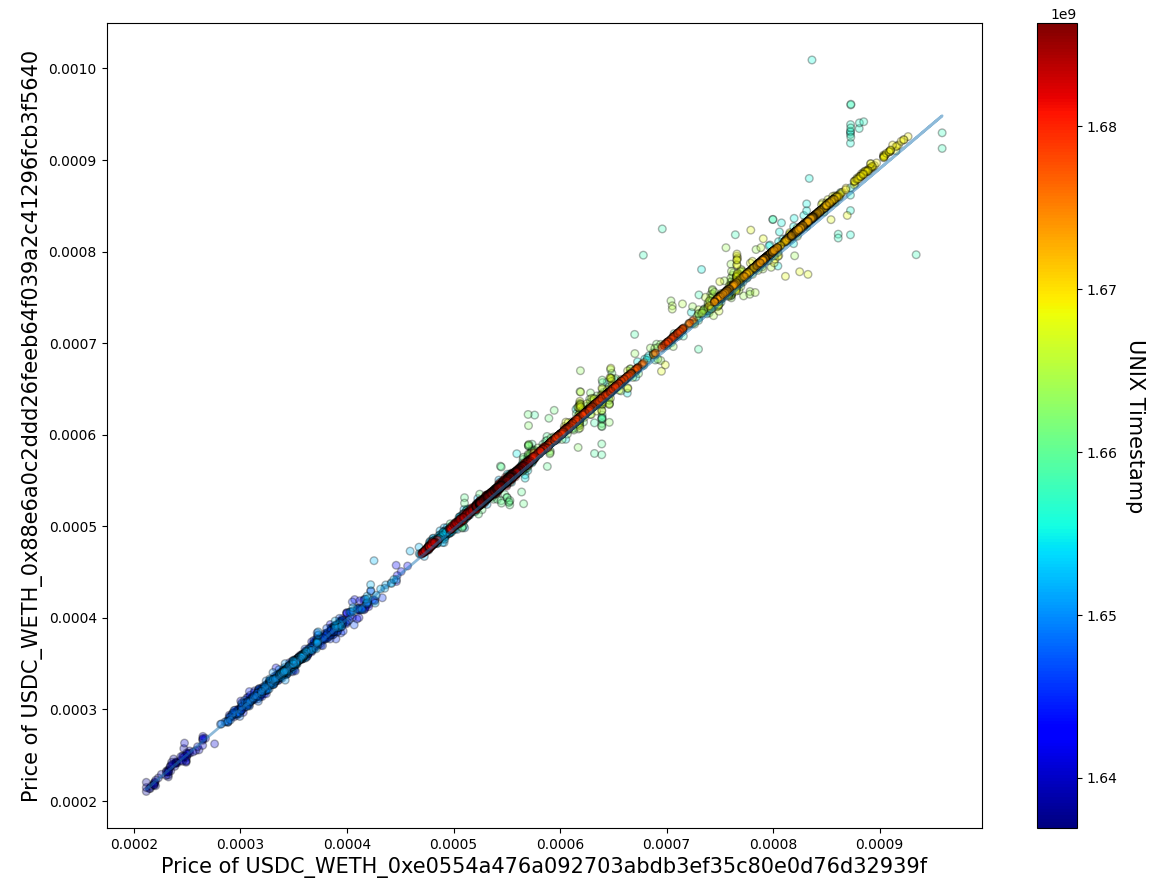
\includegraphics[width=0.8\textwidth]{project/Images/simple_hedge_ratio.png}
    \caption{Conducting OLS to obtain the Hedge Ratio \label{fig:f1}}
\end{figure}

\section{Sliding Window OLS Strategy}
As mentioned earlier, the hedge ratio plays a crucial role in minimizing risk and achieving a market-neutral position in trading strategies. However, employing a static hedge ratio may prove suboptimal since market conditions and the correlation between paired assets can evolve over time. To tackle this challenge, a dynamic approach is adopted using a sliding window approach. In this approach, the hedge ratio is continuously updated at each tick by considering the most recent data. The length of the data window used for the calculation is determined by the value specified in the \texttt{window\_size} argument. By incorporating the sliding window mechanism, the hedge ratio remains adaptive to the changing market dynamics, providing a more accurate and responsive estimation for effective risk management and trading decisions.

\section{Lagged OLS Strategy}
A lagged strategy was also implemented as an extension of the sliding window strategy. In the context of the sliding window strategy, the hedge ratio is updated using the most recent data within a specified window size. However, due to potential delays or lags in the synchronization of liquidity pools, the instantaneous prices of the assets may not fully reflect their actual relationship. Therefore, this approach aims to account for potential lags in the synchronization of liquidity pools. The lagged strategy extends the existing sliding window approach by using \texttt{sm.tsa.lagmat} function to perform the lag, which is then used to perform OLS.

\section{Unrestricted Model from the Granger Causality Test}
Similarly, to account for lag and causality, a strategy that was employed was using the Granger Causality Test. The Granger Causality Test is a statistical hypothesis test that assesses the predictive value of one time series in forecasting another. The Granger causality test is based on the idea that if variable X is causing variable Y, then the past values of X should contain information that helps predict the future values of Y beyond what can be predicted by using only the past values of Y itself. The test involves fitting two regression models: the restricted model and the unrestricted model. In the restricted model, only the past values of the dependent variable are used as predictors. In the unrestricted model, both the past values of the dependent variable and the potentially causal variable are included as predictors. By comparing the performance of these two models, the test determines whether the inclusion of the potentially causal variable improves the predictive power.
\\[3mm]
In order to estimate the hedge ratio, the unrestricted model's regression parameters are used as it captures the potential influence of the potentially causal variable on the dependent variable beyond what can be explained by the lagged values of the dependent variable alone.

\section{Kalman Filter Strategy}
Another method that is often used to ensure market-neutral positions is the use of Kalman Filters as a dynamic tool to update and adapt the hedge ratio, taking into account the changing market conditions and the evolving relationship between the paired assets. This allows for a more responsive and adaptive approach to maintaining a market-neutral position. The Kalman Filter takes into consideration not only the current price data but also the historical information and the underlying dynamics of the assets. It provides a more robust and accurate estimation of the optimal hedge ratio, which aligns with the mean reversion strategy's objective of capturing potential price divergences and profiting from their eventual convergence.
\\[3mm]
The Kalman Filter works by iteratively updating and refining its estimate of the system state using a prediction step and an update step. For this, an initial `guess' of the parameters that I use is the using Ordinary Least Squares from the historical information provided. The remainder of the parameters that are selected can be seen below:
\begin{lstlisting}[language=Python]
model = sm.OLS(price_history_2, sm.add_constant(price_history_1))
initial_state = model.fit().params[::-1]

kf = KalmanFilter(
    n_dim_state=2,
    initial_state_mean=initial_state,
    transition_matrices=np.eye(2),
    observation_matrices=obs_mat,
    transition_covariance=1e-5 * np.eye(2)
    )
\end{lstlisting}

\noindent Below describes the reasoning behind the choices of parameters:
\begin{itemize}
    \item \texttt{n\_dim\_state} - This parameter to the number of elements in the state. In our scenario, the state consists of two components: the y-intercept and the gradient.
    \item \texttt{initial\_state\_mean} - As mentioned earlier, the Kalman Filter utilizes past estimates to iteratively estimate the true states. Therefore, the OLS method is employed to calculate the initial state of the price history's regression, which returns both the y-intercept and gradient.
    \item \texttt{observation\_matrices} - The observation matrix defines the relationship between the observed measurements and the hidden state variables. Thus takes, the historical data that is provided is zipped along with 1 as the observed measurements directly correspond to the hedge ratio. This can be represented as $\begin{bmatrix} y_1 & 1 \\ y_1 & 1 \\ \vdots & 1 \\ y_n & 1\end{bmatrix}$.
    \item \texttt{transition\_matrices} - In the context of our strategy, we anticipate a consistent long-term hedge ratio. Therefore, we set the \texttt{transition\_matrices} parameter to $\begin{bmatrix} 1 & 0\\ 0 & 1 \end{bmatrix}$.
    \item \texttt{transition\_covariance} - Finally the transition\_covariance specifies the covariance matrix of the process noise. It represents the uncertainty or variability in the state transition; hence it is set to be very small, $\begin{bmatrix} 10^{-5} & 0\\ 0 & 10^{-5} \end{bmatrix}$.
\end{itemize}

\noindent Figures \ref{fig:evolving_hedge_ratio_kf} and \ref{fig:ratios_kf} provide visual representations of the hedge ratio's evolution over time. These figures illustrate that the hedge ratio while exhibiting subtle variations, does indeed change over the observed period. One notable event is the significant rise that occurs at the timestamp 1.655e9 or June 2022. This particular shift in the hedge ratio is likely attributed to the migration from the Proof of Work (PoW) consensus mechanism to the Proof of Stake (PoS) consensus mechanism on the Ethereum network.
\\[3mm]
During the transition from PoW to PoS, there are fundamental changes in how the Ethereum network reaches consensus and validates transactions. This change in the consensus mechanism can impact various aspects of the network, including the dynamics of the hedge ratio. It is plausible that the observed drop in the hedge ratio during the migration period reflects the adjustments and reconfiguration of the underlying mechanisms in response to the shift to PoS.

\begin{figure}[!htb]
    \centering
    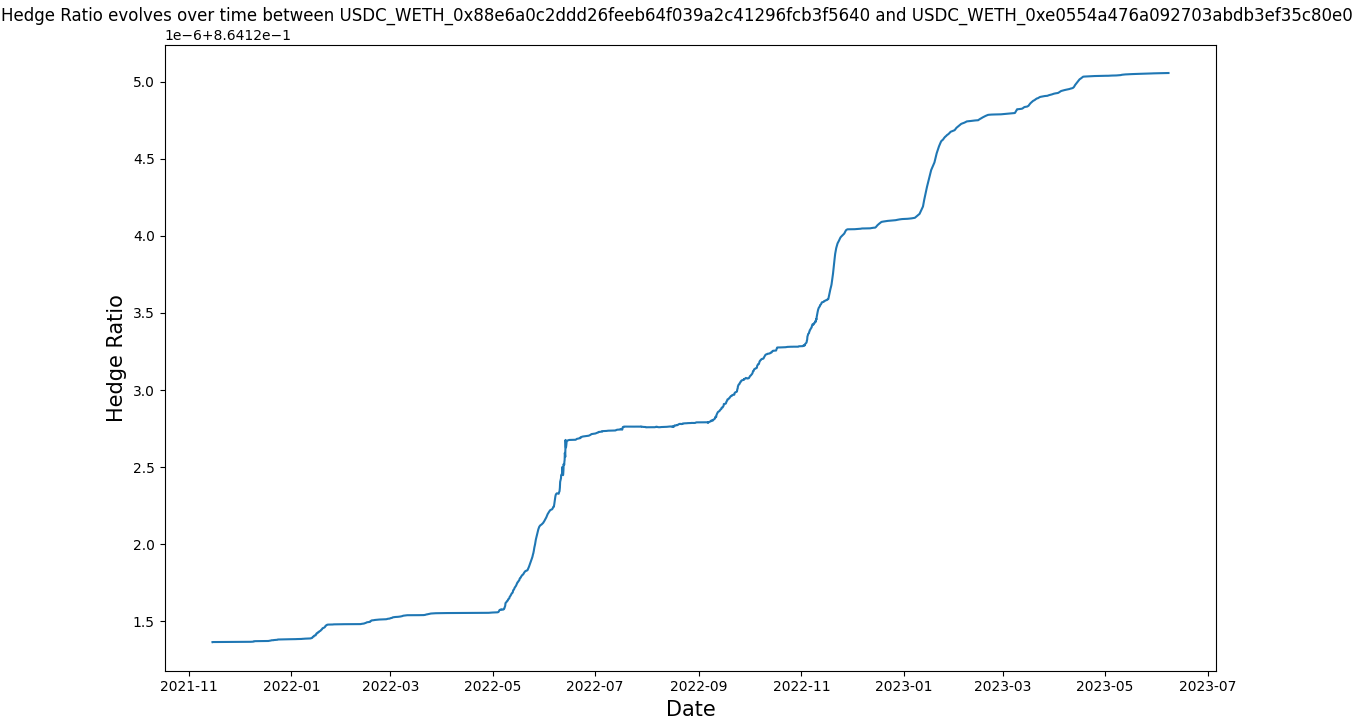
\includegraphics[width=\textwidth]{project/Images/Evolving_hedge_ratio_kf.png}
    \caption{Plot of how the Hedge Ratio using the Kalman Filter \label{fig:evolving_hedge_ratio_kf}}
\end{figure}
\vspace{-0.7cm}
\begin{figure}[!htb]
    \centering
    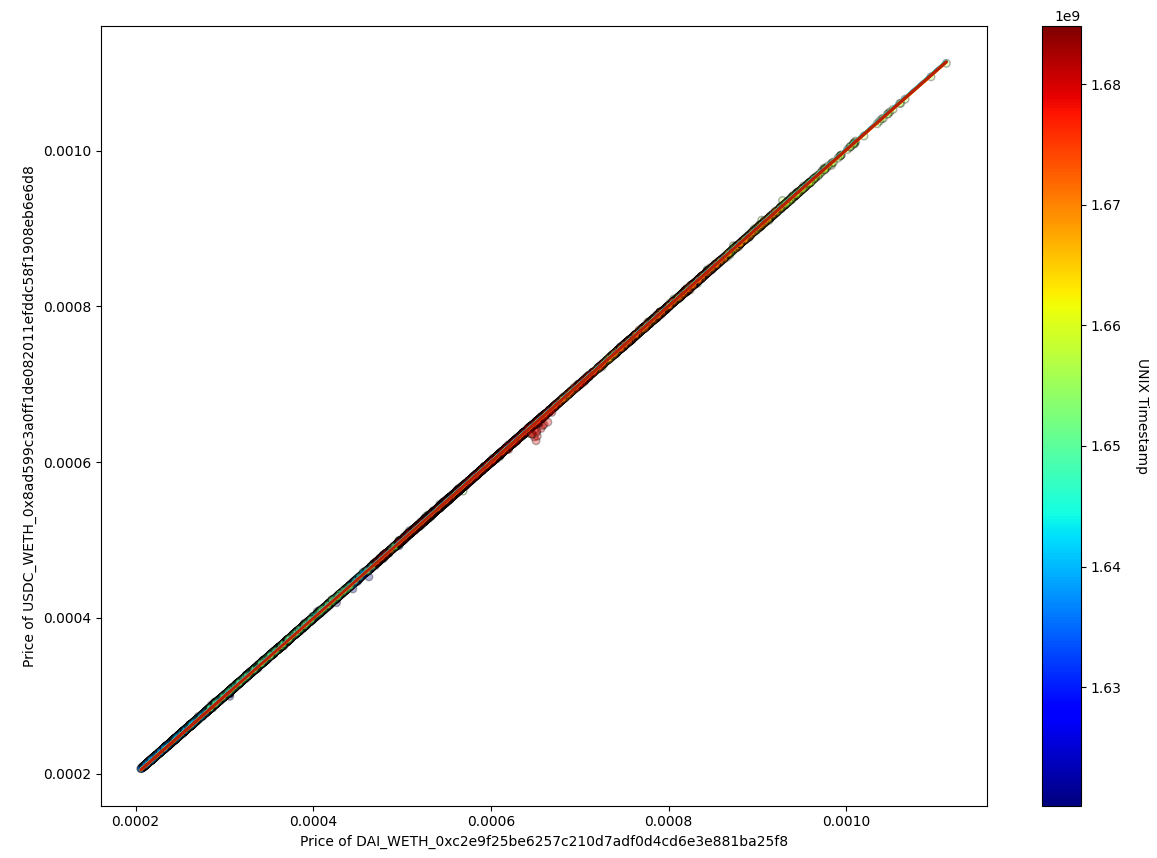
\includegraphics[width=0.7\textwidth]{project/Images/plots_1.png}
    \caption{The plot shows the Kalman Filter estimating the regression line over time, \label{fig:ratios_kf}}
\end{figure}

